\documentclass[journal,12pt,twocolumn]{IEEEtran}
%
\usepackage{setspace}
\usepackage{gensymb}
%\doublespacing
\singlespacing

%\usepackage{graphicx}
%\usepackage{amssymb}
%\usepackage{relsize}
\usepackage[cmex10]{amsmath}
%\usepackage{amsthm}
%\interdisplaylinepenalty=2500
%\savesymbol{iint}
%\usepackage{txfonts}
%\restoresymbol{TXF}{iint}
%\usepackage{wasysym}
\usepackage{amsthm}
%\usepackage{iithtlc}
\usepackage{mathrsfs}
\usepackage{txfonts}
\usepackage{stfloats}
\usepackage{bm}
\usepackage{cite}
\usepackage{cases}
\usepackage{subfig}
%\usepackage{xtab}
\usepackage{longtable}
\usepackage{multirow}
%\usepackage{algorithm}
%\usepackage{algpseudocode}
\usepackage{enumitem}
\usepackage{mathtools}
\usepackage{steinmetz}
\usepackage{tikz}
\usepackage{circuitikz}
\usepackage{verbatim}
\usepackage{tfrupee}
\usepackage[breaklinks=true]{hyperref}
%\usepackage{stmaryrd}
\usepackage{tkz-euclide} % loads  TikZ and tkz-base
%\usetkzobj{all}
\usetikzlibrary{calc,math}
\usepackage{listings}
    \usepackage{color}                                            %%
    \usepackage{array}                                            %%
    \usepackage{longtable}                                        %%
    \usepackage{calc}                                             %%
    \usepackage{multirow}                                         %%
    \usepackage{hhline}                                           %%
    \usepackage{ifthen}                                           %%
  %optionally (for landscape tables embedded in another document): %%
    \usepackage{lscape}     
\usepackage{multicol}
\usepackage{chngcntr}
%\usepackage{enumerate}

%\usepackage{wasysym}
%\newcounter{MYtempeqncnt}
\DeclareMathOperator*{\Res}{Res}
%\renewcommand{\baselinestretch}{2}
\renewcommand\thesection{\arabic{section}}
\renewcommand\thesubsection{\thesection.\arabic{subsection}}
\renewcommand\thesubsubsection{\thesubsection.\arabic{subsubsection}}

\renewcommand\thesectiondis{\arabic{section}}
\renewcommand\thesubsectiondis{\thesectiondis.\arabic{subsection}}
\renewcommand\thesubsubsectiondis{\thesubsectiondis.\arabic{subsubsection}}

% correct bad hyphenation here
\hyphenation{op-tical net-works semi-conduc-tor}
\def\inputGnumericTable{}                                 %%

\lstset{
%language=C,
frame=single, 
breaklines=true,
columns=fullflexible
}
%\lstset{
%language=tex,
%frame=single, 
%breaklines=true
%}

\begin{document}
%


\newtheorem{theorem}{Theorem}[section]
\newtheorem{problem}{Problem}
\newtheorem{proposition}{Proposition}[section]
\newtheorem{lemma}{Lemma}[section]
\newtheorem{corollary}[theorem]{Corollary}
\newtheorem{example}{Example}[section]
\newtheorem{definition}[problem]{Definition}
%\newtheorem{thm}{Theorem}[section] 
%\newtheorem{defn}[thm]{Definition}
%\newtheorem{algorithm}{Algorithm}[section]
%\newtheorem{cor}{Corollary}
\newcommand{\BEQA}{\begin{eqnarray}}
\newcommand{\EEQA}{\end{eqnarray}}
\newcommand{\define}{\stackrel{\triangle}{=}}
\bibliographystyle{IEEEtran}
%\bibliographystyle{ieeetr}
\providecommand{\mbf}{\mathbf}
\providecommand{\pr}[1]{\ensuremath{\Pr\left(#1\right)}}
\providecommand{\qfunc}[1]{\ensuremath{Q\left(#1\right)}}
\providecommand{\sbrak}[1]{\ensuremath{{}\left[#1\right]}}
\providecommand{\lsbrak}[1]{\ensuremath{{}\left[#1\right.}}
\providecommand{\rsbrak}[1]{\ensuremath{{}\left.#1\right]}}
\providecommand{\brak}[1]{\ensuremath{\left(#1\right)}}
\providecommand{\lbrak}[1]{\ensuremath{\left(#1\right.}}
\providecommand{\rbrak}[1]{\ensuremath{\left.#1\right)}}
\providecommand{\cbrak}[1]{\ensuremath{\left\{#1\right\}}}
\providecommand{\lcbrak}[1]{\ensuremath{\left\{#1\right.}}
\providecommand{\rcbrak}[1]{\ensuremath{\left.#1\right\}}}
\theoremstyle{remark}
\newtheorem{rem}{Remark}
\newcommand{\sgn}{\mathop{\mathrm{sgn}}}
\providecommand{\abs}[1]{\left\vert#1\right\vert}
\providecommand{\res}[1]{\Res\displaylimits_{#1}} 
\providecommand{\norm}[1]{\left\lVert#1\right\rVert}
%\providecommand{\norm}[1]{\lVert#1\rVert}
\providecommand{\mtx}[1]{\mathbf{#1}}
\providecommand{\mean}[1]{E\left[ #1 \right]}
\providecommand{\fourier}{\overset{\mathcal{F}}{ \rightleftharpoons}}
%\providecommand{\hilbert}{\overset{\mathcal{H}}{ \rightleftharpoons}}
\providecommand{\system}{\overset{\mathcal{H}}{ \longleftrightarrow}}
	%\newcommand{\solution}[2]{\textbf{Solution:}{#1}}
\newcommand{\solution}{\noindent \textbf{Solution: }}
\newcommand{\cosec}{\,\text{cosec}\,}
\providecommand{\dec}[2]{\ensuremath{\overset{#1}{\underset{#2}{\gtrless}}}}
\newcommand{\myvec}[1]{\ensuremath{\begin{pmatrix}#1\end{pmatrix}}}
\newcommand{\mydet}[1]{\ensuremath{\begin{vmatrix}#1\end{vmatrix}}}
%\numberwithin{equation}{section}
\numberwithin{equation}{subsection}
%\numberwithin{problem}{section}
%\numberwithin{definition}{section}
\makeatletter
\@addtoreset{figure}{problem}
\makeatother
\let\StandardTheFigure\thefigure
\let\vec\mathbf
%\renewcommand{\thefigure}{\theproblem.\arabic{figure}}
\renewcommand{\thefigure}{\theproblem}
%\setlist[enumerate,1]{before=\renewcommand\theequation{\theenumi.\arabic{equation}}
%\counterwithin{equation}{enumi}
%\renewcommand{\theequation}{\arabic{subsection}.\arabic{equation}}
\def\putbox#1#2#3{\makebox[0in][l]{\makebox[#1][l]{}\raisebox{\baselineskip}[0in][0in]{\raisebox{#2}[0in][0in]{#3}}}}
     \def\rightbox#1{\makebox[0in][r]{#1}}
     \def\centbox#1{\makebox[0in]{#1}}
     \def\topbox#1{\raisebox{-\baselineskip}[0in][0in]{#1}}
     \def\midbox#1{\raisebox{-0.5\baselineskip}[0in][0in]{#1}}
\vspace{3cm}
\title{Assignment 5}
\author{Shivangi Parashar}
%\title{
%	\logo{Matrix Analysis through Octave}{\begin{center}\includegraphics[scale=.24]{tlc}\end{center}}{}{HAMDSP}
%}
% paper title
% can use linebreaks \\ within to get better formatting as desired
%\title{Matrix Analysis through Octave}
%
%
% author names and IEEE memberships
% note positions of commas and nonbreaking spaces ( ~ ) LaTeX will not break
% a structure at a ~ so this keeps an author's name from being broken across
% two lines.
% use \thanks{} to gain access to the first footnote area
% a separate \thanks must be used for each paragraph as LaTeX2e's \thanks
% was not built to handle multiple paragraphs
%
%\author{<-this % stops a space
%\thanks{}}
%}
% note the % following the last \IEEEmembership and also \thanks - 
% these prevent an unwanted space from occurring between the last author name
% and the end of the author line. i.e., if you had this:
% 
% \author{....lastname \thanks{...} \thanks{...} }
%                     ^------------^------------^----Do not want these spaces!
%
% a space would be appended to the last name and could cause every name on that
% line to be shifted left slightly. This is one of those "LaTeX things". For
% instance, "\textbf{A} \textbf{B}" will typeset as "A B" not "AB". To get
% "AB" then you have to do: "\textbf{A}\textbf{B}"
% \thanks is no different in this regard, so shield the last } of each \thanks
% that ends a line with a % and do not let a space in before the next \thanks.
% Spaces after \IEEEmembership other than the last one are OK (and needed) as
% you are supposed to have spaces between the names. For what it is worth,
% this is a minor point as most people would not even notice if the said evil
% space somehow managed to creep in.
% The paper headers
%\markboth{Journal of \LaTeX\ Class Files,~Vol.~6, No.~1, January~2007}%
%{Shell \MakeLowercase{\textit{et al.}}: Bare Demo of IEEEtran.cls for Journals}
% The only time the second header will appear is for the odd numbered pages
% after the title page when using the twoside option.
% 
% *** Note that you probably will NOT want to include the author's ***
% *** name in the headers of peer review papers.                   ***
% You can use \ifCLASSOPTIONpeerreview for conditional compilation here if
% you desire.
% If you want to put a publisher's ID mark on the page you can do it like
% this:
%\IEEEpubid{0000--0000/00\$00.00~\copyright~2007 IEEE}
% Remember, if you use this you must call \IEEEpubidadjcol in the second
% column for its text to clear the IEEEpubid mark.
% make the title area
\maketitle
\newpage
%\tableofcontents
\bigskip
\renewcommand{\thefigure}{\theenumi}
\renewcommand{\thetable}{\theenumi}
%\renewcommand{\theequation}{\theenumi}
%\begin{abstract}
%%\boldmath
%In this letter, an algorithm for evaluating the exact analytical bit error rate  (BER)  for the piecewise linear (PL) combiner for  multiple relays is presented. Previous results were available only for upto three relays. The algorithm is unique in the sense that  the actual mathematical expressions, that are prohibitively large, need not be explicitly obtained. The diversity gain due to multiple relays is shown through plots of the analytical BER, well supported by simulations. 
%
%\end{abstract}
% IEEEtran.cls defaults to using nonbold math in the Abstract.
% This preserves the distinction between vectors and scalars. However,
% if the journal you are submitting to favors bold math in the abstract,
% then you can use LaTeX's standard command \boldmath at the very start
% of the abstract to achieve this. Many IEEE journals frown on math
% in the abstract anyway.
% Note that keywords are not normally used for peerreview papers.
%\begin{IEEEkeywords}
%Cooperative diversity, decode and forward, piecewise linear
%\end{IEEEkeywords}
% For peer review papers, you can put extra information on the cover
% page as needed:
% \ifCLASSOPTIONpeerreview
% \begin{center} \bfseries EDICS Category: 3-BBND \end{center}
% \fi
%
% For peerreview papers, this IEEEtran command inserts a page break and
% creates the second title. It will be ignored for other modes.
%\IEEEpeerreviewmaketitle
\vspace{2ex}
\begin{center}
%{\underline{\Large \bf Determinant}}
\end{center}
\begin{abstract}
This document explains the the concept of finding  two straight lines from given second degree equation 
\end{abstract}
Download all python codes from 
%
\begin{lstlisting}
https://github.com/shivangi-975/EE5609-Matrix_Theory/tree/master/Assignment5/Codes
\end{lstlisting}
%
Download latex-tikz codes from 
%
\begin{lstlisting}
https://github.com/shivangi-975/EE5609-Matrix_Theory/blob/master/Assignment3/Assignment5.tex
\end{lstlisting}
%
\section{Problem}
Find the value of k such that $x^2+\frac{10}{3}(xy)+y^2 -5x -7y + k =0$ represent pairs of straight lines.
\section{Theory}
The general equation of second degree is given by 
\begin{align} 
	ax^2 + 2bxy + cy^2 + 2dx + 2ey + f = 0 
\end{align}
and can be expressed as 
\begin{align}
	\vec{x}^T\vec{Vx} + 2\vec{u}^T\vec{x} + f = 0 \label{eq:eq1}
\end{align}
where 
\begin{align}
	\vec{V} = \vec{V}^T = \myvec{a & b\\b & c} \label{eq:eq2} \\
	\vec{u}^T = \myvec{d & e} \label{eq:eq3}
\end{align}
Let the pair of straight lines be given by 
\begin{align}
	\vec{n}_1^T\vec{x} = c_1\\
	\vec{n}_2^T\vec{x} = c_2
\end{align}
Equating their product with \eqref{eq:eq1}, we get
\begin{align}
	(\vec{n}_1^T\vec{x} - c_1)(\vec{n}_2^T\vec{x} - c_2) \nonumber \\
	\implies \vec{x}^T\vec{Vx} + 2\vec{u}^T\vec{x} + f = 0 \label{eq:eq4}
\end{align}
\eqref{eq:eq4} represents a pair of straight lines if
\begin{align} \label{eq:det1}
	\mydet{\vec{V} & \vec{u} \\ \vec{u}^T & f} = 0
\end{align}
\section{Solution}
Given,
\begin{align}
x^{2}+ \frac{10}{3}(xy)+y^2 -5x -7y + k =0 \label{eq:eq5}
\end{align}
Equating  \eqref{eq:eq5} to \eqref{eq:eq1}, we get
\begin{align}
	\vec{V} = \myvec{1& \frac{5}{3} \\ \frac{5}{3} & 1}\label{myeq}\\
	\vec{u}^T = \myvec{\frac{-5}{2} & \frac{-7}{2}}\label{df}
\end{align}
Substituting $\vec{V}$ and $\vec{u}^T$ in \eqref{eq:det1}, we obtain
\begin{align}\label{dett}
\mydet{1& \frac{5}{3} & \frac{-5}{2} \\ \frac{5}{3} & 1 & \frac{-7}{2} \\ \frac{-5}{2} & \frac{-7}{2} & k} = 0 \\
\implies \brak{k - \brak{\frac{49}{4}}}-\frac{5}{3}\brak{\frac{5}{3}k - \frac{35}{4}} \nonumber\\
-
\frac{5}{2} \brak{\frac{-35}{6}+\frac{5}{2}} = 0\\
\implies \frac{64}k{36} - \frac{128}{12} = 0\\
\implies \boxed{k = 6} \label{eq:result}
\end{align}
Substituting \eqref{eq:result} in \eqref{eq:eq5}, we get
\begin{align}
	x^{2}+ \frac{10}{3}(xy)+y^2 -5x -7y + 6 =0  \label{eq:reseq}
\end{align}
Hence value of k=6 represents pair of straight lines.
\section{Graphical Illustration}
Substituting value of k =6 in equation (\ref{dett})
\begin{align}
\delta&=\begin{array}{|ccc|}
1 &\frac{5}{3}& \frac{-5}{2}\\\frac{5}{3} & 1 & \frac{-7}{2}\\ \frac{-5}{2} & \frac{-7}{2} & 6
\end{array}&
\intertext{Simplyfying  the above determinant , we get}
\delta&=0
\end{align}
Since equation \eqref{eq:det1} is satisfied, we could say that the given equation \eqref{eq:reseq} represents two straight lines
\begin{align}
    \det(V)&=\begin{array}{|cc|}
1&\frac{5}{3}\\\frac{5}{3} & 1
\end{array}<0
\end{align}
Since $\det(V)<0$  lines would intersect each other
\renewcommand{\thefigure}{1}
\begin{figure}[h]
    \centering
    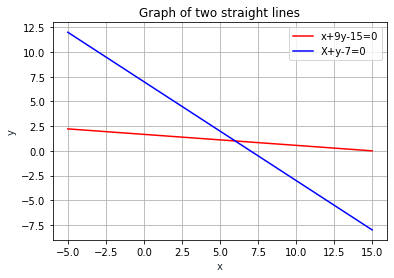
\includegraphics[width=\columnwidth]{assignment5.png}
    \caption{Pair of straight lines}
    \label{Fig :1}
\end{figure}
pair of straight lines in vector form is :
\begin{align}
    \vec{n_1}^T\vec{x}&=c_1\label{m1}\\
    \vec{n_2}^T\vec{x}&=c_2\label{m2}
\end{align}
Equating their product with \eqref{eq:eq4}
\begin{align}
(\vec{n_1}^T\vec{x}-c_1)(\vec{n_2}^T\vec{x}-c_2) &=\vec{x}^T\myvec{1 & \frac{5}{3} \\\frac{5}{3} & 1}\vec{x}\notag\\
+2\myvec{\frac{-5}{2} & \frac{-7}{2}}\vec{x}+6\label{86}
\end{align}
\begin{align}
    \vec{n_1}*\vec{n_2}&=\{1,\frac{10}{3},1\}\label{conv}\\
    c_2\vec{n_1}+c_1\vec{n_2}&=-2\myvec{\frac{-5}{2}\\\frac{-7}{2}}\label{eq98}\\
    c_1c_2&=6
\end{align}
The slopes of the lines are given by the roots of the polynomial 
\begin{align}
    &cm^2+2bm+a=0\label{e}\\
    \implies m_i&=\frac{-b\pm{\sqrt{-\det(V)}}}{c}\\
    \vec{n_i}&=k\myvec{-m_i\\1}
\end{align}
Substituting  in above equations \eqref{e} we get,
\begin{align}
    &m^2+\frac{10}{3}m+1=0\\
    &\implies m_i=\frac{\frac{-7}{2}\pm{\sqrt{-(\frac{-529}{4})}}}{-10}\label{m}
\end{align}
Solving equation \eqref{m} we have ,
\begin{align}
    m_1&=\frac{-1}{3}\\
    m_2&=-3\\
    \vec{n_1}&=k_1\myvec{\frac{1}{3}\\1}\label{n1}\\
    \vec{n_2}&=k_2\myvec{{3}\\1}\label{n2}
\end{align}
Substituting equations \eqref{n1}, \eqref{n2} in equation \eqref{conv} we get 
\begin{align}
    k_1k_2&=1
\end{align}
Possible combination of ($k_1,k_2$) is (1,1)
Lets assume $k_1=1$, $k_2=1$, we get 
\begin{align}
    \vec{n_1}&=\myvec{\frac{1}{3} \\1}\label{n11}\\
    \vec{n_2}&=\myvec{3\\1}\label{n22}
\end{align}
From equation \eqref{eq98} we get 
\begin{align}
    \myvec{\vec{n_1} & \vec{n_2}}\myvec{c_2\\c_1}&=-2\myvec{\frac{-5}{2}\\\frac{-7}{2}}\\
    \myvec{1& 3\\1 & 1}\myvec{c_2\\c_1}&=-2\myvec{\frac{-5}{2}\\\frac{-7}{2}}\\
    \frac{1}{3}c_2+3c_1&=5\label{1}\\
    c_2+c_1&=7\label{2}
\end{align}
Solving equations \eqref{1} ,\eqref{2} we get 
\begin{align}
    c_1&=1\\
    c_2&=6
\end{align}
Equations \eqref{m1}, \eqref{m2} in vector form
\begin{align}
    \myvec{\frac{1}{3}& 1}\vec{x}&=5\\
    \myvec{3 & 1}\vec{x}&=7
\end{align}
\end{document}

   
